\documentclass[10pt,notitlepage]{article}
\usepackage{graphicx} 
\usepackage{verbatim} 
\usepackage[portuguese]{babel} 
\usepackage[utf8]{inputenc}
\usepackage[hmargin=2cm,vmargin=3.5cm,bmargin=2cm]{geometry}


\begin{document}

%%%CAPA%%%
\begin{titlepage}
\begin{figure}
\centering

\includegraphics[scale=0.5]{logo.pdf}
\end{figure}



\begin{center}

Escola de Engenharia \\~  Departamento de Informática \\~ \\~ Licenciatura em Engenharia Informática \\~ \\~ \\~  \\~ \\~ \\~ \\~ \\~ \\~ \\~  


{\Huge Projecto Java - FitnessUM }
\\~ \\~ \\~ \\
Programação Orientada aos Objectos
  \vfill

\begin{figure}[h]
\centering

\end{figure}

\begin{figure}[h]
\centering
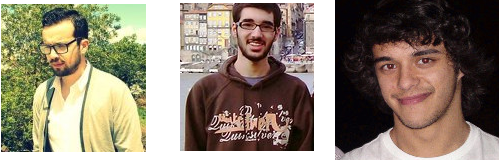
\includegraphics[scale=0.6]{autores.png}
\end{figure}

69854 ~~~~~~~~~~~~~~~~~~ 66822 ~~~~~~~~~~~~~~~~~~ 69303   \\~  João Mano ~~~~~~~~ Miguel Guimarães ~~~~~~~~ Bruno Torres  \\~ \\~ \\~ \\~ \\~ \\~ Braga, Junho de 2014
\end{center}
\end{titlepage}




\tableofcontents

\newpage


\section{Estrutura da aplicação}

\subsection{Actividades}
Para a nossa aplicação foram criadas seguintes actividades:
\begin{itemize}
\item 
\item
\item
\item
\item
\item
\item
\item
\item
\item
\item 
\item
\item
\item
\item
\item
\item
\item
\item

\end{itemize}
Para a implementação das actividades optou-se pela seguinte estrutura:
%\\%
\begin{figure}[h]
\centering
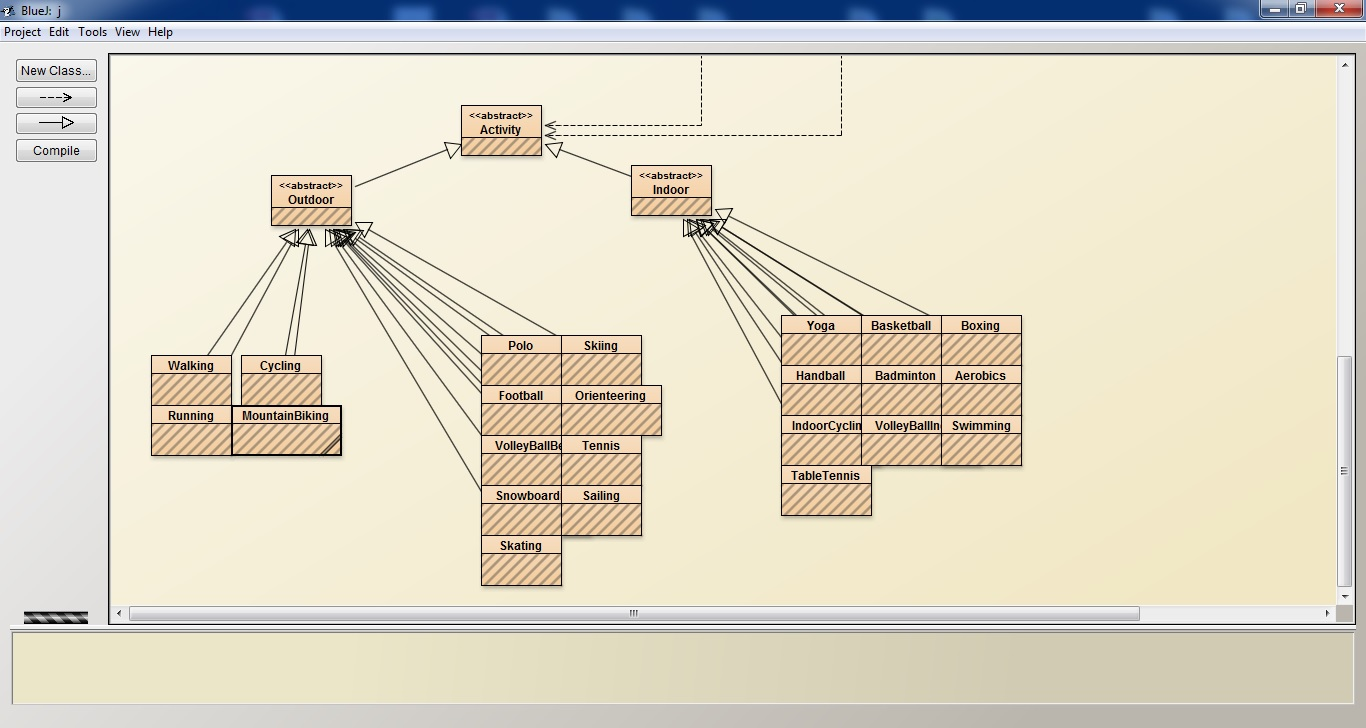
\includegraphics[scale=0.5]{Activity.jpg}
\end{figure}

\subsubsection{Classe abstracta Activity}

Esta é a classe mais abstrata, que tem a fundação de todas as actividadades desta aplicação. Contém variáveis comuns a todas as actividades, \textit{name}, \textit{date}, \textit{timeSpent} e \textit{calories} tal como os construtores, \textit{getters} e  \textit{setters}.




\subsection{Classe Abstracta Person}

Aqui usámos mais uma classe abstracta para definir todas as pessoas que usam a aplicação (Administradores ou utilizadores normais). As variáveis comuns aos todos os tipos de pessoas são \textit{email}, \textit{password}, \textit{name}, \textit{gender}, e \textit{dateOfBirth}. Para além de 
construtores, \textit{getters} e \textit{setters} esta classe não tem métodos auxiliares.





\subsection{Classe abstracta Event}

Classe com o conceito mais abstracto de Evento, contém as variáveis \textit{name}, \textit{tipoActivity}, \textit{location}, \textit{maxParticipants}, \textit{participants}, \textit{deadline}, \textit{date}, \textit{duration}, \textit{participantsList}, \textit{ranking}, \textit{desistentes} e \textit{simula}, respetivos \textit{getters} e \textit{setters} e os vários contrutores. Ainda tem métodos auxiliares para adicionar um \textit{User}, \textit{ranking}, 


\subsection{}


\end{document}

















